% ============================================================
\chapter{Ensembles Convexes}
\label{ch:ensembles}
% ============================================================

Imaginez que vous tendez un \'elastique entre deux punaises plant\'ees dans
un morceau de carton. L'\'elastique suit une ligne droite. Maintenant,
imaginez que la r\'egion accessible du carton est contrainte~: si, quelle
que soit la position des deux punaises \emph{dans} la r\'egion, l'\'elastique
reste enti\`erement dans la r\'egion, alors cette r\'egion est
\emph{convexe}. C'est une id\'ee aussi vieille que la g\'eom\'etrie
elle-m\^eme --- Euclide connaissait les polygones convexes --- mais ses
cons\'equences en optimisation sont profondes et n'ont \'et\'e pleinement
exploit\'ees qu'au XX\ieme{} si\`ecle, par des pionniers comme
Minkowski, Fenchel, Rockafellar et Boyd.

% ------------------------------------------------------------
\section{Introduction et motivation}
% ------------------------------------------------------------

Les ensembles convexes constituent la brique fondamentale de l'optimisation convexe.
Un probl\`eme d'optimisation est dit convexe lorsque l'on minimise une fonction convexe
sur un ensemble convexe. La g\'eom\'etrie de ces ensembles d\'etermine la structure
des solutions et guide la conception des algorithmes.

\begin{intuition}
Un ensemble est convexe si, pour tout couple de points de l'ensemble, le segment
les reliant est enti\`erement contenu dans l'ensemble. Cette propri\'et\'e simple
a des cons\'equences profondes~: tout minimum local est global, et les techniques
de s\'eparation par hyperplans deviennent possibles.
\end{intuition}

\section{D\'efinitions fondamentales}

\begin{definition}[Ensemble convexe]
Un ensemble $C \subseteq \R^n$ est \emph{convexe} si, pour tout $x, y \in C$ et tout
$\theta \in [0,1]$~:
\[
    \theta x + (1-\theta)y \in C.
\]
\end{definition}

\begin{definition}[Combinaison convexe]
Un point $x$ est une \emph{combinaison convexe} des points $x_1, \ldots, x_k$ s'il
existe $\theta_1, \ldots, \theta_k \geq 0$ avec $\sum_{i=1}^k \theta_i = 1$ tels que~:
\[
    x = \sum_{i=1}^k \theta_i x_i.
\]
\end{definition}

\begin{definition}[Enveloppe convexe]
L'\emph{enveloppe convexe} d'un ensemble $S \subseteq \R^n$, not\'ee $\mathrm{conv}(S)$,
est l'ensemble de toutes les combinaisons convexes de points de $S$~:
\[
    \mathrm{conv}(S) = \left\{ \sum_{i=1}^k \theta_i x_i \;\middle|\;
    x_i \in S, \; \theta_i \geq 0, \; \sum_{i=1}^k \theta_i = 1, \; k \in \N^* \right\}.
\]
\end{definition}

\begin{theoreme}[Carath\'eodory]
\label{thm:caratheodory}
Soit $S \subseteq \R^n$. Tout point de $\mathrm{conv}(S)$ peut s'\'ecrire comme
combinaison convexe d'au plus $n+1$ points de $S$.
\end{theoreme}

\begin{proof}
Soit $x \in \mathrm{conv}(S)$. Alors $x = \sum_{i=1}^k \theta_i x_i$ avec
$\theta_i > 0$, $\sum \theta_i = 1$, $x_i \in S$. Si $k > n+1$, les vecteurs
$x_2 - x_1, \ldots, x_k - x_1$ sont au nombre de $k-1 > n$, donc lin\'eairement
d\'ependants. Il existe $\mu_2, \ldots, \mu_k$ non tous nuls tels que
$\sum_{i=2}^k \mu_i (x_i - x_1) = 0$. Posons $\mu_1 = -\sum_{i=2}^k \mu_i$.
Alors $\sum_{i=1}^k \mu_i x_i = 0$ et $\sum_{i=1}^k \mu_i = 0$.

Pour $t \in \R$, $x = \sum_{i=1}^k (\theta_i - t\mu_i)x_i$. Choisissons
$t^* = \min_{i:\mu_i>0} \theta_i/\mu_i$. Alors $\theta_i - t^*\mu_i \geq 0$
pour tout $i$, et au moins un coefficient s'annule, r\'eduisant le nombre de termes.
On it\`ere jusqu'\`a $k \leq n+1$.
\end{proof}

\section{Exemples d'ensembles convexes}

\begin{exemple}[Ensembles convexes classiques]
Les ensembles suivants sont convexes~:
\begin{enumerate}
    \item \textbf{Hyperplan}~: $\{x \in \R^n \mid \inner{a}{x} = b\}$ avec $a \neq 0$.
    \item \textbf{Demi-espace}~: $\{x \in \R^n \mid \inner{a}{x} \leq b\}$.
    \item \textbf{Boule euclidienne}~: $B(x_0, r) = \{x \mid \norm{x - x_0} \leq r\}$.
    \item \textbf{Ellipso\"ide}~: $\{x \mid (x-x_0)^T P^{-1}(x-x_0) \leq 1\}$, $P \succ 0$.
    \item \textbf{Poly\`edre}~: $\{x \mid Ax \leq b, \; Cx = d\}$.
    \item \textbf{Simplexe}~: $\Delta_n = \{x \in \R^n_+ \mid \sum x_i = 1\}$.
    \item \textbf{C\^one SDP}~: $\mathbb{S}^n_+ = \{X \in \mathbb{S}^n \mid X \succeq 0\}$.
\end{enumerate}
\end{exemple}

\begin{proof}[V\'erification pour la boule]
Soient $x, y \in B(x_0, r)$ et $\theta \in [0,1]$. Par l'in\'egalit\'e triangulaire~:
\[
    \norm{\theta x + (1-\theta)y - x_0}
    = \norm{\theta(x-x_0) + (1-\theta)(y-x_0)}
    \leq \theta\norm{x-x_0} + (1-\theta)\norm{y-x_0}
    \leq \theta r + (1-\theta)r = r.
\]
\end{proof}

\section{C\^ones convexes}

\begin{definition}[C\^one]
Un ensemble $K \subseteq \R^n$ est un \emph{c\^one} si pour tout $x \in K$ et tout
$\lambda \geq 0$, on a $\lambda x \in K$.
\end{definition}

\begin{definition}[C\^one convexe]
Un c\^one $K$ est \emph{convexe} si $K$ est un ensemble convexe, ce qui \'equivaut \`a~:
pour tout $x, y \in K$ et $\lambda, \mu \geq 0$~:
\[
    \lambda x + \mu y \in K.
\]
\end{definition}

\begin{definition}[C\^one dual]
Le \emph{c\^one dual} de $K$ est~:
\[
    K^* = \{y \in \R^n \mid \inner{y}{x} \geq 0, \; \forall x \in K\}.
\]
\end{definition}

\begin{proposition}[Propri\'et\'es du c\^one dual]
\label{prop:cone_dual}
\begin{enumerate}
    \item $K^*$ est un c\^one convexe ferm\'e.
    \item Si $K_1 \subseteq K_2$, alors $K_2^* \subseteq K_1^*$.
    \item Si $K$ est un c\^one convexe ferm\'e, alors $K^{**} = K$.
\end{enumerate}
\end{proposition}

\begin{exemple}[C\^ones duaux classiques]
\begin{itemize}
    \item Le c\^one dual de $\R^n_+$ est $\R^n_+$ (auto-dual).
    \item Le c\^one dual du c\^one de Lorentz
    $\mathcal{L}^n = \{(x,t) \in \R^{n-1} \times \R \mid \norm{x} \leq t\}$
    est $\mathcal{L}^n$ lui-m\^eme.
    \item Le c\^one dual de $\mathbb{S}^n_+$ est $\mathbb{S}^n_+$.
\end{itemize}
\end{exemple}

\section{Op\'erations pr\'eservant la convexit\'e}

\begin{theoreme}[Op\'erations convexes]
\label{thm:operations}
Les op\'erations suivantes pr\'eservent la convexit\'e~:
\begin{enumerate}
    \item \textbf{Intersection}~: si $C_\alpha$ est convexe pour tout $\alpha \in I$,
          alors $\bigcap_{\alpha \in I} C_\alpha$ est convexe.
    \item \textbf{Image affine}~: si $C$ est convexe et $f(x) = Ax + b$, alors
          $f(C) = \{Ax + b \mid x \in C\}$ est convexe.
    \item \textbf{Image inverse affine}~: si $C$ est convexe, alors
          $f^{-1}(C) = \{x \mid Ax + b \in C\}$ est convexe.
    \item \textbf{Somme de Minkowski}~: si $C_1, C_2$ sont convexes, alors
          $C_1 + C_2 = \{x + y \mid x \in C_1, y \in C_2\}$ est convexe.
    \item \textbf{Projection}~: si $C \subseteq \R^n \times \R^m$ est convexe, alors
          $\{x \in \R^n \mid \exists y, (x,y) \in C\}$ est convexe.
    \item \textbf{Fonction perspective}~: si $C$ est convexe et $P(x,t) = x/t$ pour
          $t > 0$, alors $P(C)$ est convexe.
\end{enumerate}
\end{theoreme}

\begin{proof}[Preuve de (1)]
Soient $x, y \in \bigcap_\alpha C_\alpha$ et $\theta \in [0,1]$. Pour tout $\alpha$,
$x, y \in C_\alpha$, donc $\theta x + (1-\theta)y \in C_\alpha$ par convexit\'e de
$C_\alpha$. Ainsi $\theta x + (1-\theta)y \in \bigcap_\alpha C_\alpha$.
\end{proof}

\begin{remarque}
L'union de deux ensembles convexes n'est g\'en\'eralement pas convexe.
Par exemple, $\{0\} \cup \{1\}$ n'est pas convexe dans $\R$.
L'intersection arbitraire pr\'eserve la convexit\'e, mais pas l'union.
\end{remarque}

\section{Th\'eor\`emes de s\'eparation}

\begin{theoreme}[S\'eparation par hyperplan]
\label{thm:separation}
Soient $C, D \subseteq \R^n$ deux ensembles convexes non vides disjoints.
Il existe $a \in \R^n$, $a \neq 0$, et $b \in \R$ tels que~:
\[
    \inner{a}{x} \leq b \; \forall x \in C
    \quad \text{et} \quad
    \inner{a}{x} \geq b \; \forall x \in D.
\]
\end{theoreme}

\begin{theoreme}[S\'eparation stricte]
\label{thm:separation_stricte}
Soient $C$ un ensemble convexe ferm\'e non vide et $x_0 \notin C$.
Il existe $a \in \R^n$, $a \neq 0$, et $b \in \R$ tels que~:
\[
    \inner{a}{x_0} > b > \inner{a}{x} \quad \forall x \in C.
\]
\end{theoreme}

\begin{proof}
Soit $\bar{x} = \mathrm{proj}_C(x_0)$ la projection de $x_0$ sur $C$ (qui existe
et est unique car $C$ est convexe ferm\'e). Posons $a = x_0 - \bar{x}$ et
$b = \inner{a}{\bar{x}} + \frac{1}{2}\norm{a}^2$.

Pour tout $x \in C$, la caract\'erisation de la projection donne~:
\[
    \inner{x_0 - \bar{x}}{x - \bar{x}} \leq 0,
\]
c'est-\`a-dire $\inner{a}{x} \leq \inner{a}{\bar{x}}$. De plus~:
\[
    \inner{a}{x_0} = \inner{a}{\bar{x}} + \norm{a}^2 > \inner{a}{\bar{x}} + \tfrac{1}{2}\norm{a}^2 = b > \inner{a}{\bar{x}} \geq \inner{a}{x}.
\]
\end{proof}

\begin{intuition}
G\'eom\'etriquement, le th\'eor\`eme de s\'eparation affirme qu'on peut toujours
placer un hyperplan entre deux ensembles convexes disjoints. C'est l'analogue en
dimension sup\'erieure du fait qu'on peut s\'eparer deux intervalles disjoints sur
la droite r\'eelle par un point.
\end{intuition}

\section{Hyperplan d'appui}

\begin{definition}[Hyperplan d'appui]
Soit $C \subseteq \R^n$ un ensemble convexe. Un \emph{hyperplan d'appui} de $C$
en un point fronti\`ere $x_0 \in \partial C$ est un hyperplan $H = \{x \mid \inner{a}{x} = b\}$
tel que~:
\[
    \inner{a}{x_0} = b \quad \text{et} \quad
    \inner{a}{x} \leq b \; \forall x \in C.
\]
\end{definition}

\begin{theoreme}[Existence d'hyperplans d'appui]
Soit $C$ un ensemble convexe non vide avec int\'erieur non vide, et $x_0 \in \partial C$.
Alors il existe un hyperplan d'appui de $C$ en $x_0$.
\end{theoreme}

\section{Fonction d'appui et fonction indicatrice}

\begin{definition}[Fonction d'appui]
La \emph{fonction d'appui} d'un ensemble $C$ est~:
\[
    \sigma_C(y) = \sup_{x \in C} \inner{y}{x}.
\]
\end{definition}

\begin{definition}[Fonction indicatrice convexe]
La \emph{fonction indicatrice} (au sens de l'analyse convexe) de $C$ est~:
\[
    \iota_C(x) = \begin{cases} 0 & \text{si } x \in C, \\ +\infty & \text{sinon.} \end{cases}
\]
\end{definition}

\begin{proposition}
Si $C$ est convexe ferm\'e non vide, alors $\iota_C$ est convexe, propre et
semi-continue inf\'erieurement. De plus, $\sigma_C = \iota_C^*$ (la conjugu\'ee de
Fenchel de $\iota_C$).
\end{proposition}

\section{Projection sur un convexe ferm\'e}

\begin{theoreme}[Projection convexe]
\label{thm:projection}
Soit $C \subseteq \R^n$ un ensemble convexe ferm\'e non vide. Pour tout $y \in \R^n$,
il existe un unique $\bar{x} \in C$ tel que~:
\[
    \bar{x} = \argmin_{x \in C} \norm{x - y}^2.
\]
Ce point, not\'e $\mathrm{proj}_C(y)$, est caract\'eris\'e par~:
\[
    \bar{x} \in C \quad \text{et} \quad
    \inner{y - \bar{x}}{x - \bar{x}} \leq 0, \quad \forall x \in C.
\]
\end{theoreme}

\begin{proof}
\textbf{Existence.} Soit $d = \inf_{x \in C} \norm{x - y}$. Prenons $(x_k) \subset C$
avec $\norm{x_k - y} \to d$. Par l'identit\'e du parall\'elogramme~:
\[
    \norm{x_k - x_l}^2 = 2\norm{x_k - y}^2 + 2\norm{x_l - y}^2 - 4\norm{\tfrac{x_k+x_l}{2} - y}^2.
\]
Comme $\frac{x_k+x_l}{2} \in C$ (convexit\'e), $\norm{\frac{x_k+x_l}{2} - y} \geq d$, donc~:
\[
    \norm{x_k - x_l}^2 \leq 2\norm{x_k - y}^2 + 2\norm{x_l - y}^2 - 4d^2 \to 0.
\]
$(x_k)$ est de Cauchy, converge vers $\bar{x} \in C$ (car $C$ est ferm\'e).

\textbf{Unicit\'e.} Si $\bar{x}_1, \bar{x}_2$ sont deux projections, le m\^eme argument
montre $\norm{\bar{x}_1 - \bar{x}_2} = 0$.

\textbf{Caract\'erisation.} $\bar{x}$ minimise $\varphi(x) = \norm{x-y}^2$ sur $C$
si et seulement si pour tout $x \in C$ et $t \in (0,1]$~:
$\varphi(\bar{x} + t(x-\bar{x})) \geq \varphi(\bar{x})$, ce qui donne
$\inner{y - \bar{x}}{x - \bar{x}} \leq 0$.
\end{proof}

\begin{proposition}[Non-expansivit\'e de la projection]
La projection $\mathrm{proj}_C$ est non expansive~:
\[
    \norm{\mathrm{proj}_C(x) - \mathrm{proj}_C(y)} \leq \norm{x - y}, \quad \forall x, y \in \R^n.
\]
En particulier, $\mathrm{proj}_C$ est continue (lipschitzienne de constante $1$).
\end{proposition}

\section{Poly\`edres et repr\'esentations}

\begin{definition}[Poly\`edre]
Un \emph{poly\`edre} est l'intersection d'un nombre fini de demi-espaces~:
\[
    P = \{x \in \R^n \mid Ax \leq b\}, \quad A \in \R^{m \times n}, \; b \in \R^m.
\]
Un poly\`edre born\'e est appel\'e \emph{polytope}.
\end{definition}

\begin{theoreme}[Minkowski--Weyl]
Un ensemble $P \subseteq \R^n$ est un polytope si et seulement s'il est l'enveloppe
convexe d'un nombre fini de points~:
\[
    P = \mathrm{conv}(\{v_1, \ldots, v_k\}).
\]
Plus g\'en\'eralement, tout poly\`edre admet une repr\'esentation de la forme~:
\[
    P = \mathrm{conv}(\{v_1, \ldots, v_k\}) + \mathrm{cone}(\{d_1, \ldots, d_l\}).
\]
\end{theoreme}

\section{Interpr\'etation g\'eom\'etrique}

\begin{center}
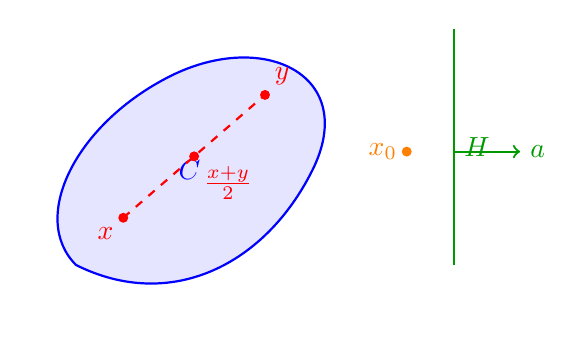
\begin{tikzpicture}[scale=1.2]
    % Convex set
    \draw[thick, blue, fill=blue!10]
        (0,0) .. controls (1,-0.5) and (2,0) ..
        (2.5,1) .. controls (3,2) and (2,2.5) ..
        (1,2) .. controls (0,1.5) and (-0.5,0.5) .. (0,0);
    \node[blue] at (1.2,1) {$C$};

    % Two points and segment
    \fill[red] (0.5,0.5) circle (1.5pt) node[below left] {$x$};
    \fill[red] (2,1.8) circle (1.5pt) node[above right] {$y$};
    \draw[red, thick, dashed] (0.5,0.5) -- (2,1.8);

    % Midpoint
    \fill[red] (1.25,1.15) circle (1.5pt) node[below right]
        {$\frac{x+y}{2}$};

    % Separating hyperplane
    \draw[thick, green!60!black] (4,0) -- (4,2.5)
        node[midway, right] {$H$};
    \fill[orange] (3.5,1.2) circle (1.5pt) node[left] {$x_0$};
    \draw[->, thick, green!60!black] (4,1.2) -- (4.7,1.2) node[right] {$a$};
\end{tikzpicture}
\end{center}

\section{Impl\'ementation Python}

\begin{codeblock}[title=\textbf{Projection sur le simplexe et v\'erification de convexit\'e}]
\begin{minted}{python}
import numpy as np
import matplotlib.pyplot as plt

def project_simplex(v):
    """Projection sur le simplexe standard."""
    n = len(v)
    u = np.sort(v)[::-1]
    cumsum = np.cumsum(u)
    rho = np.max(np.where(u + (1 - cumsum) / (np.arange(n) + 1) > 0))
    theta = (cumsum[rho] - 1) / (rho + 1)
    return np.maximum(v - theta, 0)

def is_convex_hull_member(point, vertices):
    """Verifie si point est dans conv(vertices) via LP."""
    import scipy.optimize as opt
    k = len(vertices)
    V = np.array(vertices).T  # n x k
    n = V.shape[0]
    # min 0 s.t. V @ theta = point, sum(theta) = 1, theta >= 0
    c = np.zeros(k)
    A_eq = np.vstack([V, np.ones((1, k))])
    b_eq = np.append(point, 1.0)
    bounds = [(0, None)] * k
    res = opt.linprog(c, A_eq=A_eq, b_eq=b_eq, bounds=bounds)
    return res.success

# Demonstration: projection sur le simplexe
np.random.seed(42)
v = np.random.randn(3)
p = project_simplex(v)
print(f"Point original: {v}")
print(f"Projection:     {p}")
print(f"Somme = {p.sum():.6f}, min = {p.min():.6f}")
\end{minted}
\end{codeblock}

\section{Exercices}

\begin{exercice}[$\star$]
Montrer que l'intersection de deux demi-espaces est convexe.
\end{exercice}

\begin{exercice}[$\star$]
Montrer que l'image d'un ensemble convexe par une application lin\'eaire est convexe.
\end{exercice}

\begin{exercice}[$\star\star$]
Soit $C = \{x \in \R^n \mid \norm{x}_1 \leq 1\}$. Montrer que $C$ est un polytope
et d\'eterminer ses sommets.
\end{exercice}

\begin{exercice}[$\star\star$]
Soit $C$ un ensemble convexe ferm\'e et $x_0 \notin C$. D\'emontrer qu'il existe
un unique point $\bar{x} \in C$ le plus proche de $x_0$. Montrer que
$\inner{x_0 - \bar{x}}{x - \bar{x}} \leq 0$ pour tout $x \in C$.
\end{exercice}

\begin{exercice}[$\star\star$]
Calculer le c\^one dual du c\^one de Lorentz
$\mathcal{L}^n = \{(x,t) \in \R^{n-1}\times\R \mid \norm{x} \leq t\}$.
\end{exercice}

\begin{exercice}[$\star\star\star$]
D\'emontrer le th\'eor\`eme de Carath\'eodory en dimension 2 g\'eom\'etriquement,
puis g\'en\'eraliser la preuve en dimension $n$.
\end{exercice}

\begin{exercice}[$\star\star\star$]
Soit $f : \R^n \to \R$ continue. Montrer que l'ensemble de sous-niveau
$\{x \mid f(x) \leq \alpha\}$ est ferm\'e. Donner un exemple montrant qu'il
n'est pas n\'ecessairement convexe m\^eme si $f$ est continue.
\end{exercice}
